\section{Introduzione}
\begin{frame}{Introduzione}
    \begin{itemize}
        \item Language Model (LM)
              \begin{itemize}
                  \item Sviluppo di modelli probabilistici in grado di prevedere un documento, in una collezione, data una query.
                        \[P(d|q) = \prod_{t\in q}^{ } \lambda \frac{tf(t,d)}{|d|} + (1 - \lambda) \frac{cf(t)}{cs}\]

                        \(
                        \text{Approcci di LM classici} \left\lbrace\parbox{7cm}{Latent Dirichlet allocation (LDA) \\ Latent semantic analysis (LSA)}\right.
                        \)

                        \begin{center}
                            Si propone un nuovo modello denominato\\ \underline{GENERALIZED LANGUAGE MODEL (GLM)}
                        \end{center}
              \end{itemize}
        \item Word Embedding
              \begin{itemize}
                  \item Rappresentazione delle parole in un nuovo spazio, con lo scopo di memorizzarne le informazioni semantiche e sintattiche.
              \end{itemize}
    \end{itemize}
\end{frame}

\begin{frame}{GLM}
    \underline{IDEA}

    Processo di trasformazione attraverso un <<noisy channel>> in cui un termine \(t^{'}\) viene mutato in un altro termine \(t\).

    \bigskip
    Tre approcci di trasformazione del termine:
    \begin{wrapfigure}[3]{r}{7cm}
        \centering
        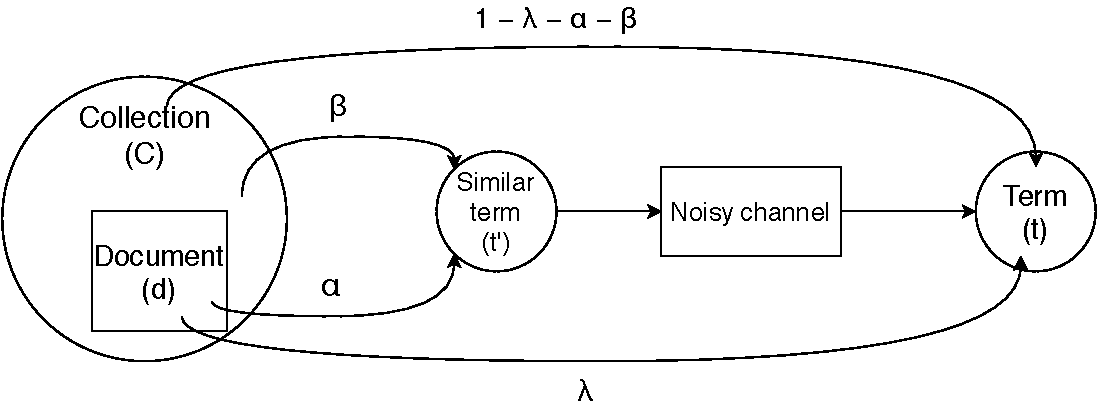
\includegraphics[width=7cm]{img/glm.pdf}
    \end{wrapfigure}
    \begin{itemize}
        \item Direct term sampling
        \item Transformation via Document
        \item Transformation via Collection
    \end{itemize}
\end{frame}

\begin{frame}{Formula GLM}
    \setlength{\abovedisplayskip}{1pt}
    \setlength{\belowdisplayskip}{1pt}
    \[
        \begin{split}
            P(t|d) & = \lambda P(t|d) + \alpha \sum_{{t}'\in d}P(t,{t}'|d)P({t}')\\
            & + \beta \sum_{{t}'\in N}P(t,{t}'|C)P({t}') + (1-\lambda-\alpha-\beta)P(t|C)
        \end{split}
    \]
    \begin{itemize}
        \item Termine \(\lambda\): Probabilità del termine \(t\) della query all'interno del documento \(d\) senza trasformazione.
        \item Termine \(\alpha\): Probabilità di trasformare i termini \({t}'\) del documento in un termine \(t\) della query.
        \item Termine \(\beta\): Probabilità di trasformare i termini \({t}'\) della collezione \(C\) in un termine \(t\) della query.
        \item Termine \(1-\lambda-\alpha-\beta\): Probabilità del termine \(t\) della query all'interno della collezione \(C\).
    \end{itemize}
\end{frame}

\begin{frame}{Trasformazione di \({t}'\) in \(t\)}

    \begin{columns}
        \begin{column}{0.5\textwidth}
            \[P(t,t'|d) = \frac{sim(t,t')}{\sum (d)}\frac{tf(t',d)}{|d|}\]
        \end{column}
        \begin{column}{0.5\textwidth}
            \[P(t,t'|C) = \frac{sim(t,t')}{\sum (Nt)}\frac{cf(t')}{cs}\]
        \end{column}
    \end{columns}

    \bigskip
    \begin{itemize}
        \item Entrambi i termini \(t\) e \({t}'\) vengono rappresentati mediante word embedding.
        \item Per il calcolo della similarità viene usata la Cosine Similarity.
    \end{itemize}

    \[sim(A,B) = cos(\vartheta ) = \frac{A * B}{\left \| A \right \| * \left \| B \right \|} = \frac{\sum_{i=1}^{n} Ai * Bi}{\sqrt{\sum_{i=1}^{n}Ai^{2}}\sqrt{\sum_{i=1}^{n}Bi^{2}}}\]

\end{frame}

\begin{frame}{Caratteristiche GLM}

    L'utilizzo del Generalized Language Model ha due vantaggi:

    \begin{itemize}
        \item Stima quanto un termine è semanticamente simile al contenuto di un documento.
        \item Colma le differenze di vocabolario tra query e documenti aggiungendo termini correlati al documento.
    \end{itemize}
\end{frame}